



\section{Data and Insights}
%\subsection{Data}

The analysis in this work is performed on two datasets from XuetangX.
XuetangX, launched in October 2013, is now one of the largest MOOC platforms in China.
%, which was launched in October 2013. 
It has provided over 1,000 courses and attracted more than 10,000,000 registered users.
% up to now.  
XuetangX has twelve categories of courses: art, biology, computer science, economics, engineering, foreign language, history, literature, math, philosophy, physics, and social science. 
%Moreover, 
Users in XuetangX can choose the learning mode: Instructor-paced Mode (IPM) and {Self-paced Mode (SPM)}.  IPM   follows the same course schedule as conventional classrooms, while in SPM, one could have more flexible schedule to study online by herself/himself. Usually an IPM course spans over 16 weeks in XuetangX, while an SPM course spans a longer period.
Each user can enroll one or more courses. When one studying a course, the system records multiple types of activities: video watching (watch, stop, and jump), forum discussion (ask questions and replies), assignment completion (with correct/incorrect answers, and reset), and web page clicking (click and close a course page).

\vpara{Two Datasets.}
%We use two datasets in this study. Both are from XuetangX.
%Our dataset includes both Instructor-paced  and Self-paced courses. We utilize two datasets in our experiments: 
The first dataset contains 39 IPM  courses and their enrolled students. It
was also used for KDDCUP 2015. Table~\ref{tab:KDDdata} lists   statistics of this dataset. With this dataset, we compare our proposed method with existing methods, as the challenge has attracted 821 teams to participate.
We refer to this dataset as KDDCUP.

The other dataset contains 698 IPM courses and 515 SPM courses. Table~\ref{tab:XuetangXdata} lists  the statistics. The dataset contains richer information, which can be used to test the robustness and generalization of the proposed method.
This dataset is referred to as XuetangX.



\begin{table}
	\centering
	\caption{Statistics of the KDDCUP dataset.}
\small
	\setlength{\tabcolsep}{3mm}{\begin{tabular}{l|l|r}
			\hline \hline
			
			Category&  Type   & Number\\
			\hline
			\multirow{3}{*}{log} & \# video activities & 1,319,032\\
			
			&  \# forum activities & 10,763,225\\
			
			& \# assignment activities & 2,089,933 \\
			
			& \# web page activities & 738,0344 \\
			\hline
			\multirow{5}{*}{enrollment} &  \# total &  200,904  \\
			
			& \# dropouts & 159,223 \\
			
			& \# completions &41,681 \\
			
			& \# users &  112,448   \\
			
			&  \# courses &    39   \\	
			\hline \hline
	\end{tabular}}
	\label{tab:KDDdata}
	\normalsize
\end{table}
\begin{table}
	\centering
	\caption{Statistics of the XuetangX dataset.}
	\small
	\begin{threeparttable}
		\setlength{\tabcolsep}{1.3mm}{\begin{tabular}{l|l|r|r}
				\hline \hline
				Category & Type   &\#IPM\tnote{*}  & \#SPM\tnote{*} \\
				\hline
				\multirow{3}{*}{log} &\# video activities & 50,678,849&  38,225,417 \\
				
				& \# forum activities & 443,554 &   90,815\\
				
				&  \# assignment activities & 7,773,245& 3,139,558 \\
				
				& \# web page activities   & 9,231,061 & 5,496,287\\
				\hline
				\multirow{5}{*}{enrollment} &  \# total  & 467,113 & 218,274\\
				
				& \# dropouts &372,088 & 205,988\\
				
				&  \# completions  & 95,025 & 12,286\\
				
				& \#  users   &254,518 & 123,719\\
				
				& \# courses   & 698& 515\\	
				\hline \hline
		\end{tabular}}
			\begin{tablenotes}
			\footnotesize
			\item[*] \#IPM and \#SPM respectively stands for the number for the corresponding IPM courses and SPM courses.%, and  represents the number of SPM courses.
		\end{tablenotes}
	\end{threeparttable}
	\label{tab:XuetangXdata}
	\normalsize
\end{table}


%\section{Observational Analysis}
%	\label{sec:analysis}
    %\subsection{Data Preprocessing}

   % In order to construct the dataset used for training model, we need to manually divide the whole course duration into $history$ period and $future$ period. Figure \ref{fig:dataCons} presents the data construction strategy. We use the first $D_h$ days after the learning starting time as the  $history$ period, while $future$ period is from $D_h+1$-st day to $(D_h+D_f)$-th day. For \textit{KDDCUP dataset} and Instructor-paced courses in \textit{XuetangX Large-Scale Dataset}, the learning starting time is defined as the course starting time, while for Self-paced courses in \textit{XuetangX Large-Scale Dataset}, we treat user's first visiting time to the course as the learning start time. For \textit{KDDCUP dataset}, $D_h$ and $D_f$ are set to $30$ and $10$ respectively by the organizers of \textit{KDDCUP 2015}. As for \textit{XuetangX Large-Scale Dataset}, we adopt different strategies for Instructor-and Self-paced courses. For Instructor-paced courses, we set $D_h=35$, $D_f=10$, while for Self-paced courses $D_h=60, D_f=10$. Since learners' behaviors in Self-paced courses exhibit more heterogeneity, the larger choice of  $D_h$'s value for Self-paced courses is to make the training data more sufficient.  
    
\subsection{Insights} 
    \label{sec:temporal}
     
\hide{
    In order to study users' different engagement patterns on XuetangX, we propose a cluster method by using users ``temporal codes'' as input, which encode a user's activities on courses into a vector. The definition is below.
}
    Before proposing our methodology, we try to gain a better understanding of the users' learning behavior.
    We first perform a clustering analysis on users' learning activities. To construct the input for the clustering analysis, we define a concept of \textit{temporal code} for each user. 
    %Formally, we have
    
    \emph{Definition 1.} \textbf{Temporal Code}:
    For each user $u$ and one of her enrolled course $c$, the temporal code is defined as a binary-valued vector $\mathbf{s}^u_{c}=[s^u_{c,1}, s^u_{c,2},..., s^u_{c,K}]$, where $s^u_{c,k} \in \{0,1\}$ indicates whether user $u$ visits course $c$ in the $k$-th week. Finally, we concatenate all course-related vectors and generate the temporal code for each user 
    as $\mathbf{S}^u=[\mathbf{s}^u_{c_1}, \mathbf{s}^u_{c_2},..., \mathbf{s}^u_{c_M}]$, where $M$ is the number of courses.
    
    Please note that the temporal code is usually very sparse. We feed the sparse representations of all users' temporal codes into a $K$-means algorithm.
    The number of clusters is set to $5$ based on a \textit{Silhouette Analysis}~\cite{rousseeuw1987silhouettes} on the data. 
    Table~\ref{tab:clusterStat} shows the clustering results. It can be  seen that 
    both cluster 2 and cluster 5 have low dropout rates, but more interesting thing is that users of cluster 5 seem to be hard workers --- with the longest video watching time, while users of cluster 2 seem to be active forum users --- the number of questions (or answers) posted by these users is almost $10\times$ higher than the others. This corresponds to different motivations that users come to MOOCs. Some users, e.g., users from cluster 5, use MOOC to seriously study knowledge, while some other users, e.g., cluster 2, may simply want to meet friends with similar interest.
    %    while the dropout rates for users in the other three clusters are much higher. We also find that the dropout probability is significantly correlated with users' activity frequency. For example, users in cluster 2 and 5 have more video activities than users in other three clusters, which indicates users in these two clusters watch more course videos. Although users in clusters 2 and  5 have a similar dropout probability, their engagement patterns are quite different. Comparing to cluster 2, users in cluster 5 have more video activities and less forum activities. This suggests that those in cluster 5 may prefer to studying by themselves, whereas those in cluster 2 are more interested in discussing with other students. 
    Another interesting phenomenon is about users in cluster 4. Their average number of revise answers for assignment (i.e.  \#reset) is much higher than all the other clusters.
    %with high dropout rate, i.e. clusters 1 and 3. 
    Users of this cluster probably are students with difficulties to learn the corresponding courses.
    %This suggests that these users may care more about their grades on MOOCs, and this may lead to the fact that their average dropout rate is lower than users in cluster 1 (0.66 vs 0.78) and cluster 3 (0.66 vs 0.83).  
    
    
    \begin{table}
    \hspace{-0.01in}
    	\centering
    	\caption{Results of clustering analysis. C1-C5 --- Cluster 1 to 5; CAR --- average correct answer ratio. }
    	\small
    	\label{tab:clusterStat}
    	\setlength{\tabcolsep}{1mm}\begin{tabular}{@{}c@{}|l@{}|c|c|c|c|c@{}}
    		\hline
    		\hline
    		Category &  Type   & C1& C2 & C3& C4&C5 \\
    		\hline
    		\multirow{3}{*}{video}&  \#watch &21.83 &46.78 &12.03&19.57 & \textbf{112.1}\\	
    		\cline{2-7}
    		& \#stop     &28.45 & 68.96&20.21&37.19& \textbf{84.15}\\
    		\cline{2-7}
    		& \#jump   &16.30 & 16.58& 11.44& 14.54& \textbf{21.39} \\
    		\hline
    		\multirow{2}{*}{forum}&  \#question & 0.04 & \textbf{0.38} &0.02 & 0.03 & 0.03 \\
    		\cline{2-7}
    		& \#answer &0.13 &\textbf{3.46}&0.13&0.12&0.17\\
    		\hline
    		\multirow{2}{*}{assignment} & CAR &0.22 & \textbf{0.76} & 0.19& 0.20 & 0.59\\
    		\cline{2-7}
    		& \#revise  &0.17 & 0.02& 0.04& \textbf{0.78}& 0.01\\
    		\hline
    		\multirow{2}{*}{session}    & seconds &1,715 &714& \textbf{1,802}& 1,764& 885\\
    		\cline{2-7}                
    		&  count     &3.61 &\textbf{8.13}& 2.18&4.01& 7.78\\ 
    		\hline
    		\multirow{2}{*}{enrollment} & \#enrollment & 21,048 & 9,063&\textbf{401,123} &25,042 & 10,837\\
    		\cline{2-7}
    		& total \#users & 2,735 & 4,131& \textbf{239,302} & 4,229 & 4,121 \\
    		\cline{2-7}
    		& dropout rate &0.78 &0.29 &\textbf{0.83} &0.66 &0.28\\
    		\hline	
    		\hline
    	\end{tabular}
    	\normalsize
    \end{table}

\hide{
    her temporal code  a course $c \in \mathbb{C}$ in the first $K$ weeks is represented as a vector code $\mathbf{s}^u_{c}=[s^u_{c,1}, s^u_{c,2},..., s^u_{c,K}]$, where $s^u_{c,k} \in \{0,1\}, (1 \le k \le K)$ represents whether $u$ visit $c$ in $k$-th week. Note that  $\mathbf{s}^u_{c}$ is set to all $0$ if $u$ has not enrolled in $c$. Then the ``temporal code'' of $u$ is obtained by concatenating all course temporal vectors: $\mathbf{S}^u=[\mathbf{s}^u_{c_1}, \mathbf{s}^u_{c_2},..., \mathbf{s}^u_{c_M}], c_m \in \mathbb{C}, $$(1 \le m \le M)$. \\


    In experiments, we use the first $5$ week logs to construct the ``temporal codes'', i.e. $K=5$. All users' ``temporal codes'' are input to a K-means algorithm for clustering users. Based on the \textit{Silhouette Analysis}, the number of clusters is set to $5$.	The statistics of $5$ clusters are described in Table \ref{tab:clusterStat}. Both clusters 2 and 5 have low dropout rates, while the dropout rates for users in the other three clusters are much higher. We also find that the dropout probability is significantly correlated with users' activity frequency. For example, users in cluster 2 and 5 have more video activities than users in other three clusters, which indicates users in these two clusters watch more course videos. Although users in clusters 2 and  5 have a similar dropout probability, their engagement patterns are quite different. Comparing to cluster 2, users in cluster 5 have more video activities and less forum activities. This suggests that those in cluster 5 may prefer to studying by themselves, whereas those in cluster 2 are more interested in discussing with other students. Another intriguing phenomenon is about users in cluster 4. Their average number of revise answers for assignment (i.e. Avg. \# reset) is much higher than the other 2 clusters with high dropout rate, i.e. clusters 1 and 3. This suggests that these users may care more about their grades on MOOCs, and this may lead to the fact that their average dropout rate is lower than users in cluster 1 (0.66 vs 0.78) and cluster 3 (0.66 vs 0.83).  
}    

    
	%\subsection{Dropout Correlation between Courses}
    
    
    \vpara{Correlation Between Courses.}
    We further study whether there is any correlation for users dropout behavior between different courses. 
    Specifically, we try to answer this question: will someone's dropout for one course increase or decrease the probability that she drops out from another course?
    %user's likelihood of dropping out in other registered courses? and \emph{How does the degree of influence change with time?} 
    %To answer these two questions, 
    We conduct a regression analysis to examine this.
    %across weeks. 
    A user's dropout behavior in a course is encoded as a 16-dim dummy vector, with each element representing whether the user has visited the course in the corresponding week (thus 16 corresponds to the 16 weeks for studying the course). The input and output of the regression model are two dummy vectors which indicate a user's dropout behavior for two different courses in the same semester. By examining the slopes of regression results (Figure~\ref{fig:courseLinreg}), we can observe a significantly positive correlation between users' dropout probabilities of different enrolled courses, 
    %across periods, 
    though overall the correlation decreases over time. 
    Moreover, we did the analysis for courses of the same category and those across different categories. It can be seen that the correlation between courses of the same category is higher than courses from different categories. 
    One potential explanation is that when a user has limited time to study MOOC, they may first give up substitutive courses instead of those with complementary knowledge domain. 
    

%As shown in Figure \ref{fig:courseLinreg} , we could observe that the dropout correlation between courses is significantly positive, i.e., \emph{if user dropout from one course, then he will more likely drop out from another course at the same time,}  and the correlation  \emph{decreases} with the passing of time in a term.  What's more, we could observe that the slopes of experiments on same category courses are larger than those of experiments on different category courses, which means that the dropout influence from same category courses is stronger than the influence from different category courses.
	
	\begin{figure}[t]
	\centering 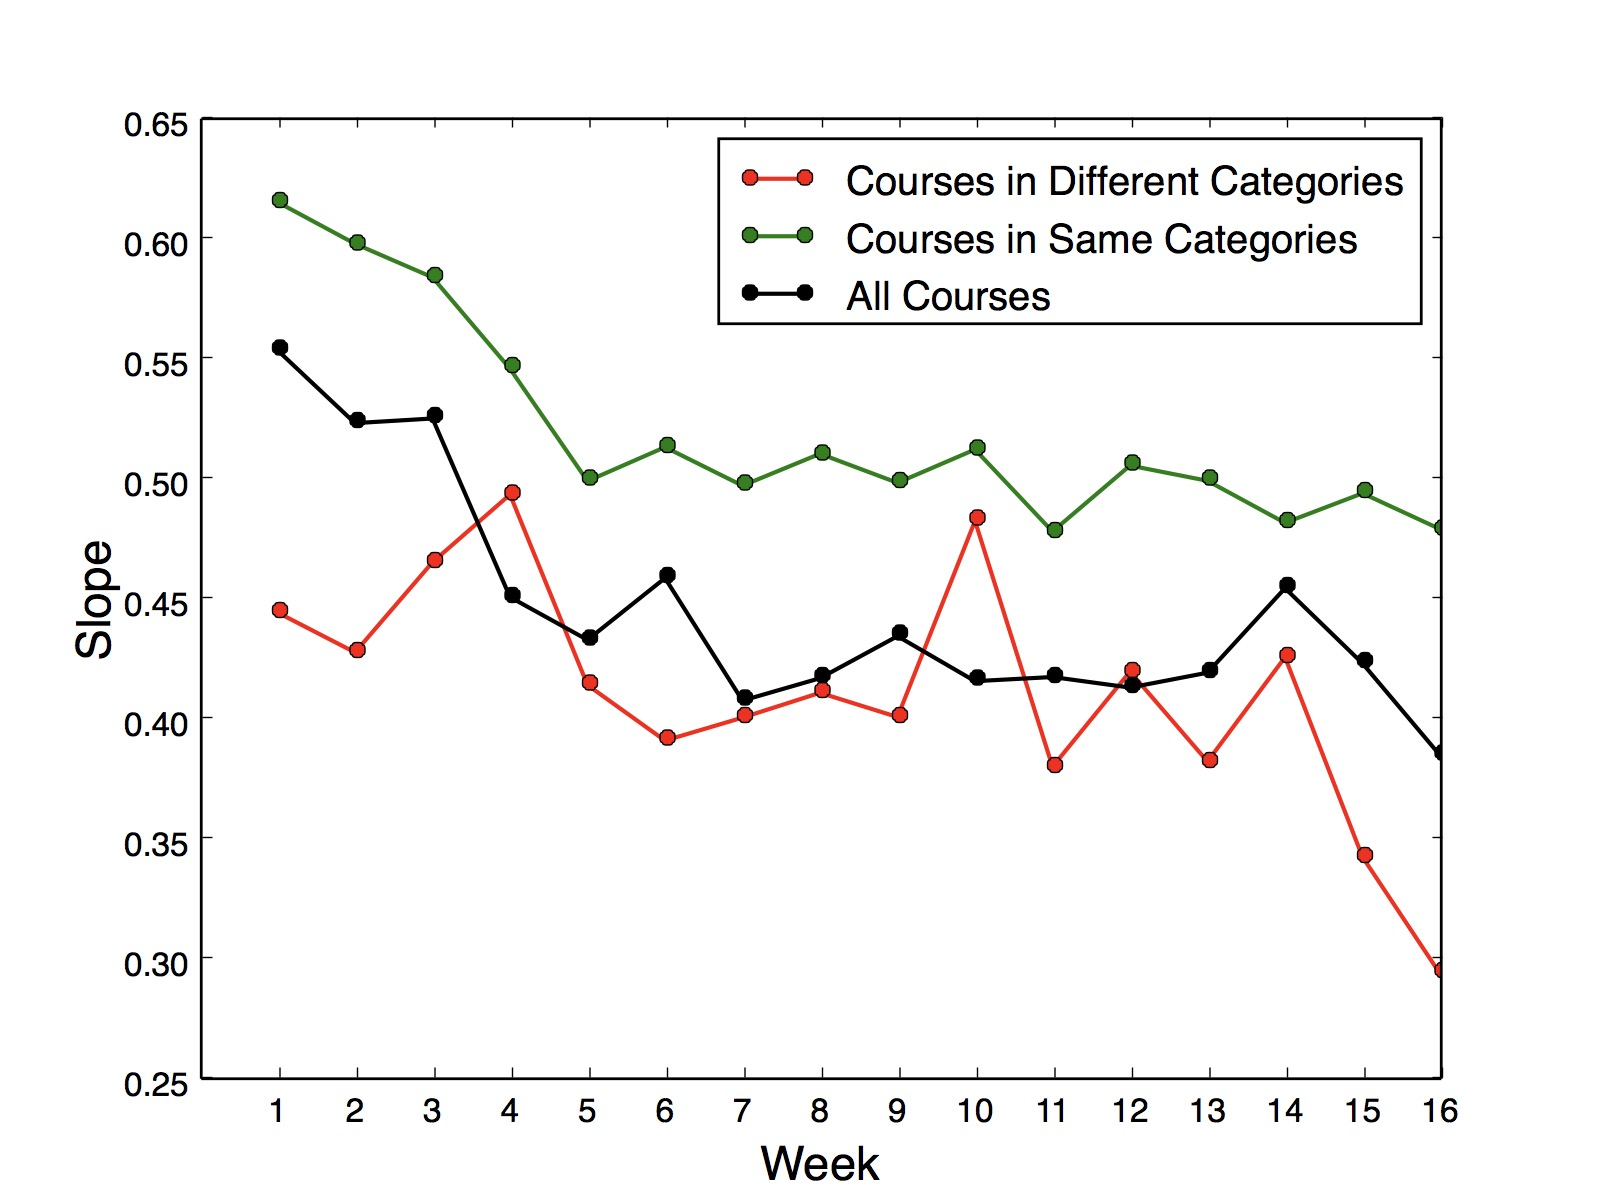
\includegraphics[ height=5cm]{lingress_slope.jpg}
	\caption{Dropout correlation analysis between courses. The $x$-axis denotes the weeks from 1 to 16 and the $y$-axis is the slope of linear regression results for dropout correlation between two different courses. The red line is the result of different category courses, the green line denotes the slope of same category courses, and the black line is pooling results in all courses.}
	\label{fig:courseLinreg}
	\end{figure}
	
	\begin{figure}[t]
	\centering
		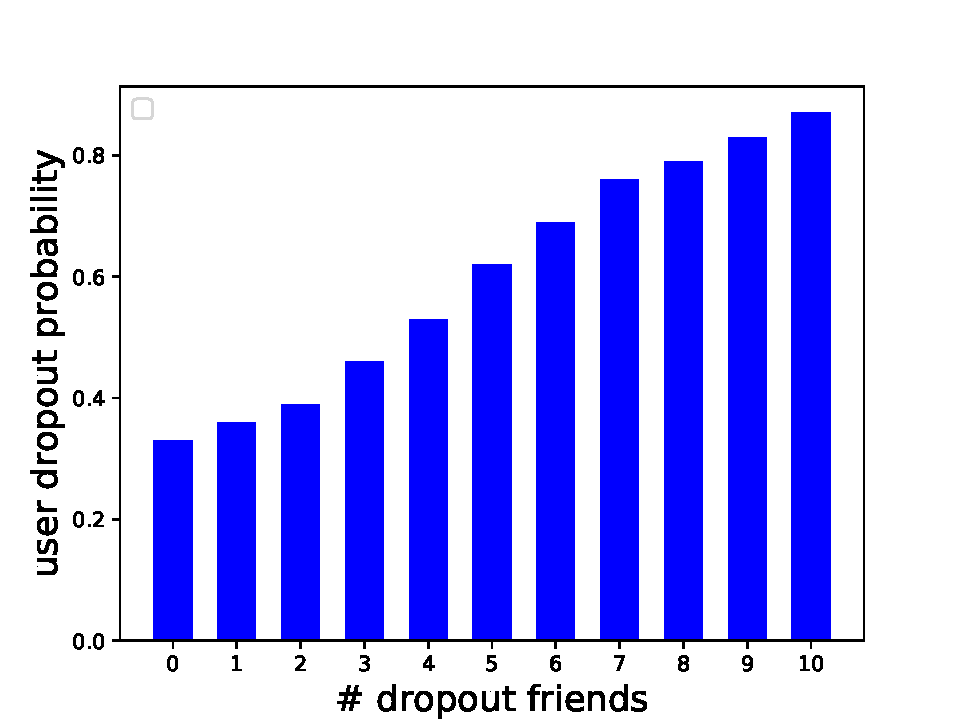
\includegraphics[height=5cm]{friends_inf.pdf}
		\caption{User dropout probability conditioned on the number of dropout friends. $x$-axis is the number of dropout friends, and $y$-axis is user's dropout probability.}
		\label{fig:friendInf}
	\end{figure}
	
	%\subsection{Influence From Dropout Friends}
    
	%\label{sec:influence}
\vpara{Influence From Dropout Friends.}
	%In real life, users' behaviors are easily affected by their friends. 
	Users' online study behavior may influence each other~\cite{Qiu:2016:MPL:2835776.2835842}. We did another analysis to understand how the influence would matter for dropout prediction.
    %In this section, we analyze the 
    %users' dropout behavior would be influenced their friends.
    In XuetangX, the friend relationship is implicitly defined using co-learning relationships. 
    More specifically, 
    %correlation between users and their friends. One bottleneck of this task is that because of the limited social activity data on MOOCs, it is difficult for us to identify the social relationship between users. Therefore, we simply assume that a user's friends are co-learning students who have similar learning interests with her, and 
    we use a network-based method to discover users' friend relationships. First, we build up a user-course bipartite graph $G_{uc} $ based on the enrollment relation.
	 %set $\mathbb{E}$. $G_{uc}$ is a bipartite graph whose 
	 The nodes are all users and courses, and the edge between user $u$ and course $c$ represents that $u$ has enrolled in course $c$. Then we use DeepWalk~\cite{Perozzi:2014:DOL:2623330.2623732}, an algorithm for learning representations of vertices in a graph, to learn a low dimensional vector for each user node and each course node in $G_{uc}$. Based on the user-specific representation vectors, we  compute the cosine similarity between  users who have enrolled a same course. Finally, those users with high similarity score, i.e., greater than 0.8, are considered as friends. 

In order to analyze the influence from dropout friends quantitatively, we calculate users' dropout probabilities conditional on the number of dropout friends.
Figure~\ref{fig:friendInf} presents the results. We see users' dropout probability increases monotonically from $0.33$ to $0.87$ when the number of dropout friends ranges from $1$ to $10$. This  indicates that a user's dropout rate is greatly influenced by her/his friends' dropout behavior.
	 
	